\section{Methodology}
\label{sec:method}

This section describes the architectural formulation of ApproxDA-TransUNet. We first outline the global lightweight topology, followed by a rigorous formulation of the tri-axial attention approximation in the ApproxDA block, the slim decoder design, and a comprehensive computational complexity analysis.

\subsection{Overall Lightweight Architecture}
Figure~\ref{fig:overall_arch} depicts the complete end-to-end architecture of ApproxDA-TransUNet. Contrasting sharply with the monolithic 108M-parameter DA-TransUNet~\cite{sun2024datransunet}, ApproxDA-TransUNet is engineered from the ground up for extreme efficiency while maintaining rich multi-scale representation capacity.

\begin{figure*}[t]
\centering
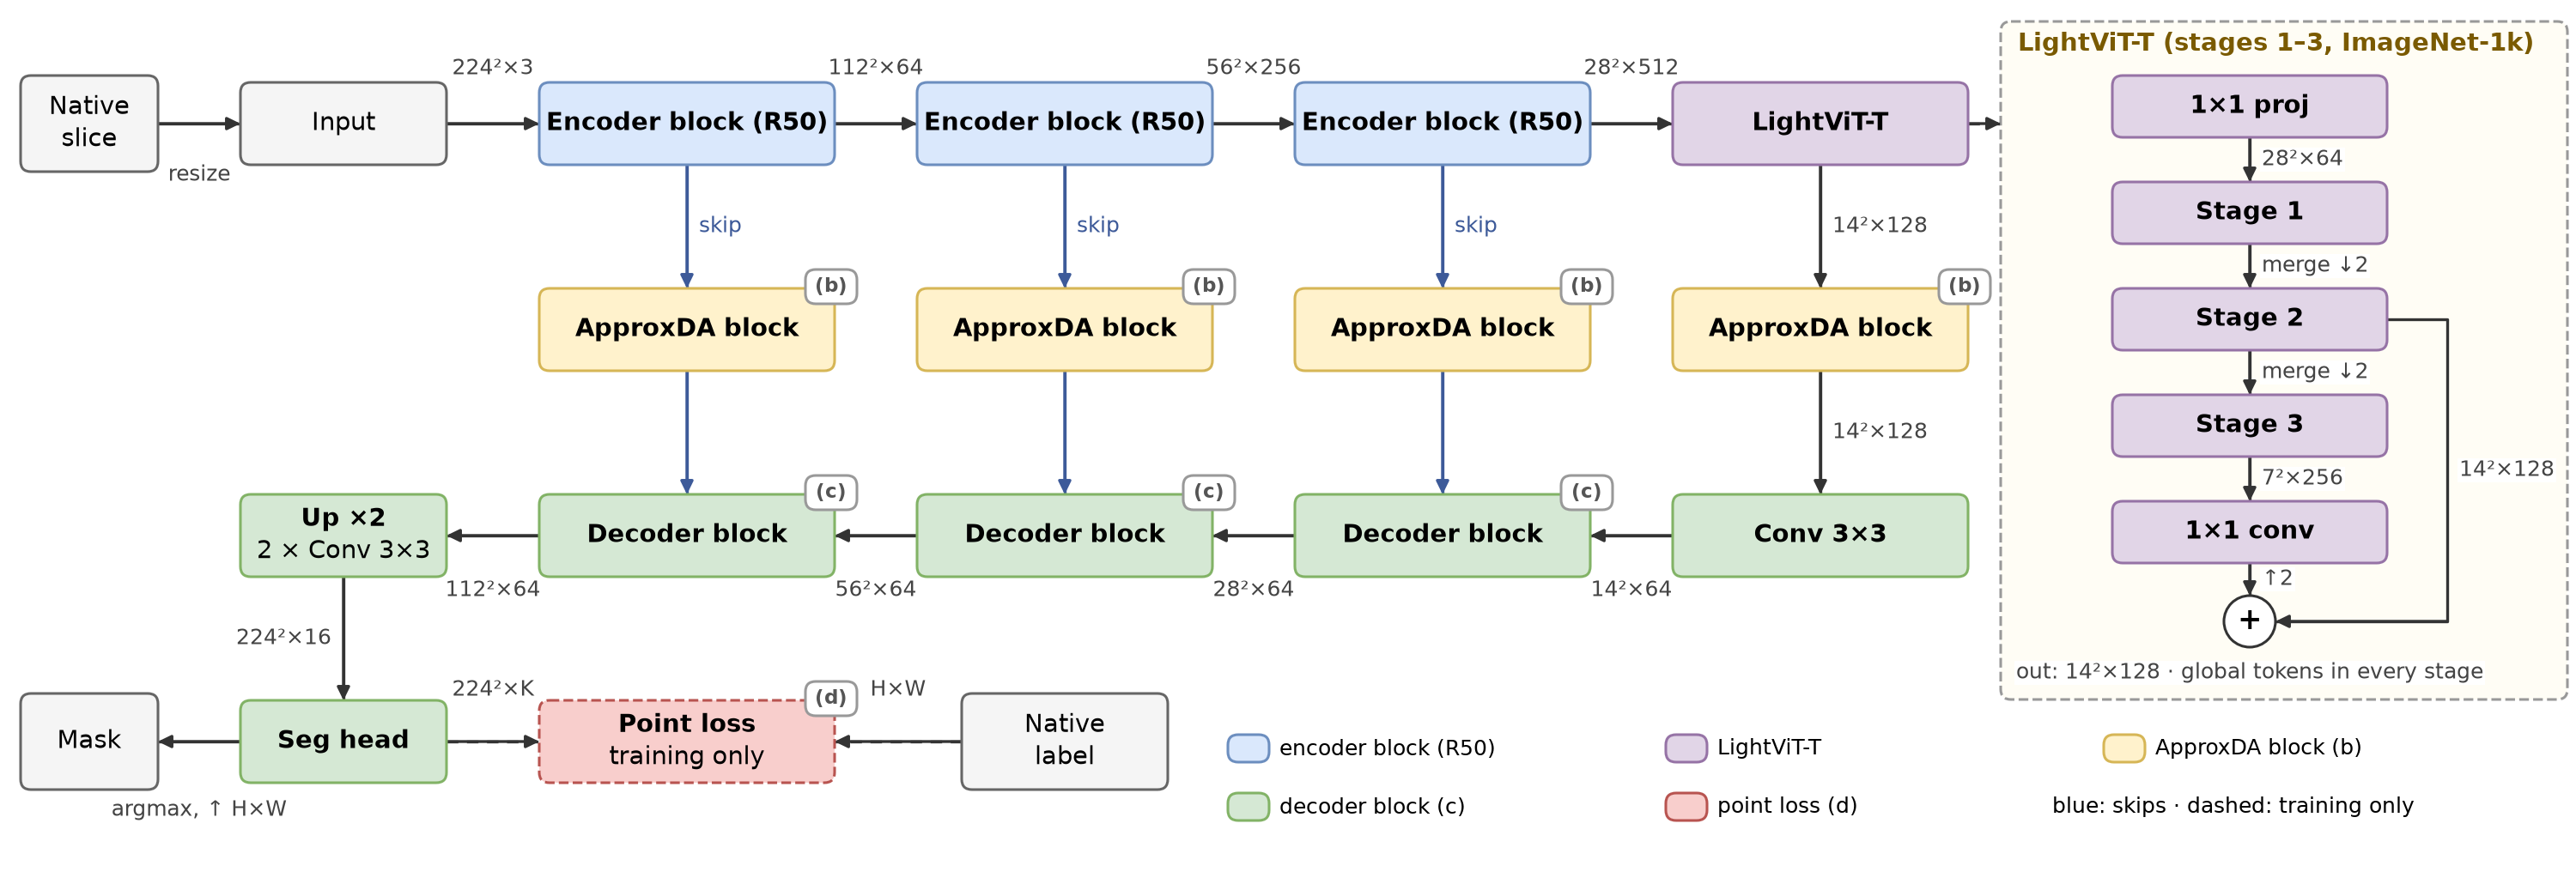
\includegraphics[width=\textwidth]{figures/approxda_light_unet_a.png}
\caption{Overall architecture of the lightweight ApproxDA-TransUNet. The encoder consists of an early-truncated ResNet-50 (Stages 1--2, down to stride 8) followed by a top-down LightViT-T bottleneck. ApproxDA blocks are uniformly placed on all three multi-scale skip connections ($1/8$, $1/4$, $1/2$) and the bottleneck. The decoder maintains a compact, uniform channel width of $C=64$, yielding a total parameter budget of only 10.75M.}
\label{fig:overall_arch}
\end{figure*}

\subsubsection{Early-Truncated CNN Stem}
In standard TransUNet and DA-TransUNet, a full ResNet-50 backbone is executed through all four stages (down to stride 16 and 1024 channels), requiring 23.5M CNN parameters. The resulting $14{\times}14$ feature map is then linearly projected to a 768-dimensional token space and processed by a 12-layer Vision Transformer (ViT-B/16), contributing an additional 86M parameters.

ApproxDA-TransUNet eliminates this massive architectural redundancy by truncating ResNet-50 immediately after Stage 2. For an input image $\mathbf{I} \in \mathbb{R}^{3 \times H \times W}$ (typically $224 \times 224$ or $256 \times 256$):
\begin{itemize}
    \item \textbf{Stem \& Stage 1}: Generates feature maps $\mathbf{F}_{1/2} \in \mathbb{R}^{64 \times \frac{H}{2} \times \frac{W}{2}}$ (stride 2) and $\mathbf{F}_{1/4} \in \mathbb{R}^{256 \times \frac{H}{4} \times \frac{W}{4}}$ (stride 4).
    \item \textbf{Stage 2}: Produces feature map $\mathbf{F}_{1/8} \in \mathbb{R}^{512 \times \frac{H}{8} \times \frac{W}{8}}$ (stride 8).
\end{itemize}
Stages 3 and 4 of ResNet-50 are entirely discarded, immediately trimming over 14M convolutional parameters.

\subsubsection{LightViT-T Bottleneck and Attention Placement}
Instead of feeding tokens into a standard isotropic ViT-B, we route $\mathbf{F}_{1/8}$ into LightViT-T~\cite{huang2022lightvit}, a hierarchical lightweight vision transformer with top-down token interactions. Operating on the stride-8 feature map ($28 \times 28$ for $224 \times 224$ input), LightViT-T sequentially transforms tokens across three stages, outputting bottleneck representation $\mathbf{Z} \in \mathbb{R}^{128 \times \frac{H}{16} \times \frac{W}{16}}$ ($14 \times 14$ resolution) with only $\approx 0.81\text{M}$ parameters. The bottleneck ApproxDA block is positioned post-transformer, directly operating on $\mathbf{Z}$ to refine global representations before decoding.

\subsection{The ApproxDA Block Formulation}
Figure~\ref{fig:approxda_block_detail} illustrates the internal topology of the ApproxDA block. The module receives input tensor $\mathbf{X} \in \mathbb{R}^{C \times H \times W}$ and splits computation into two parallel streams: Low-Rank Windowed Position Attention (PAM) and Grouped Channel Attention (CAM).

\begin{figure*}[t]
\centering
\begin{subfigure}[b]{0.64\textwidth}
    \centering
    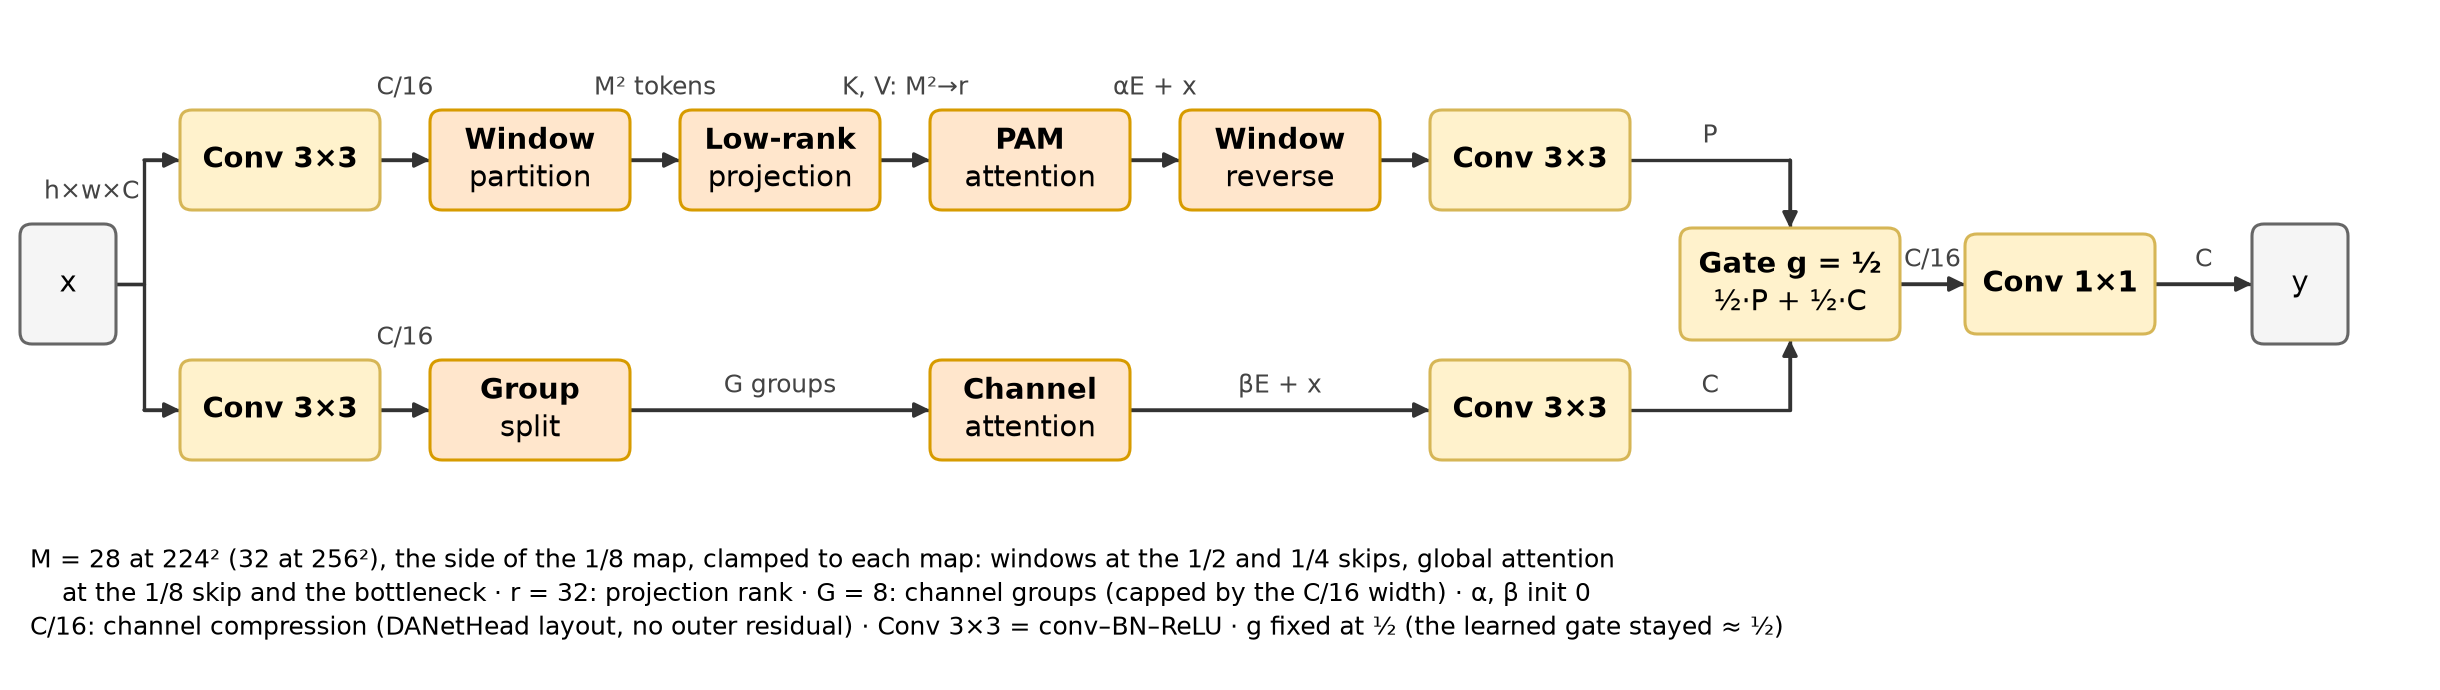
\includegraphics[width=\textwidth]{figures/approxda_light_unet_b.png}
    \caption{ApproxDA Block with tri-axial approximation ($M, r, G$) and fixed gate ($g=0.5$).}
    \label{fig:block_pam_cam}
\end{subfigure}
\hfill
\begin{subfigure}[b]{0.33\textwidth}
    \centering
    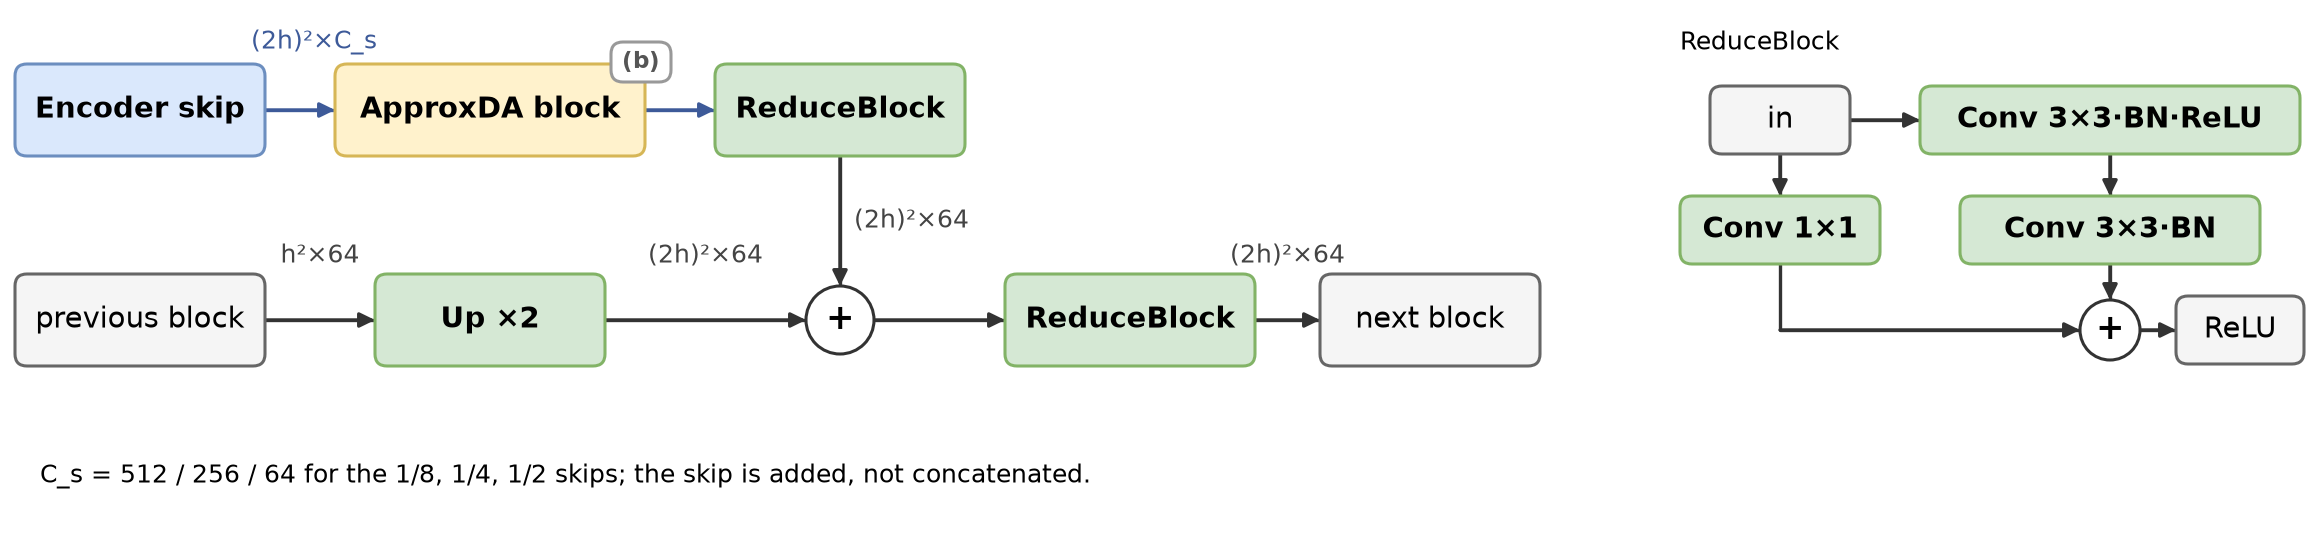
\includegraphics[width=\textwidth]{figures/approxda_light_unet_c.png}
    \caption{Slim Decoder Block ($C=64$).}
    \label{fig:block_decoder}
\end{subfigure}
\caption{Detailed architectural diagrams of (a) the ApproxDA block with Low-Rank Windowed PAM and Grouped CAM branches, and (b) the compact decoder block with uniform $C=64$ channel width.}
\label{fig:approxda_block_detail}
\end{figure*}

\subsubsection{Bottleneck Convolutional Compression}
Both branches initially pass $\mathbf{X}$ through an identical bottleneck compression:
\begin{equation}
    \mathbf{X}' = \operatorname{ReLU}(\operatorname{BN}(\operatorname{Conv}_{3\times3}(\mathbf{X}))) \in \mathbb{R}^{C' \times H \times W},
\end{equation}
where $C' = \max(8, \lfloor C/16 \rfloor)$. This reduces channel dimensionality by $16\times$, drastically diminishing the input dimensions for subsequent attention operators.

\subsubsection{Low-Rank Windowed Position Attention (PAM)}
Full spatial self-attention requires pairwise affinities between all $N = HW$ tokens, yielding $\mathcal{O}(N^2 C')$ complexity. We approximate this along two orthogonal dimensions: \textbf{spatial windowing} ($M$) and \textbf{low-rank projection} ($r$).

\paragraph{Window Partitioning} The feature map $\mathbf{X}'$ is partitioned into non-overlapping spatial windows of size $M \times M$, where $M = \min(M, H, W)$ ($M=28$ for $224 \times 224$ inputs). Consequently, the $1/2$ and $1/4$ skip stages are partitioned into $4 \times 4$ and $2 \times 2$ window grids, while the $1/8$ skip and bottleneck operate within a single global window. Within each window of $N_w = M^2$ tokens, queries $\mathbf{Q}$, keys $\mathbf{K}$, and values $\mathbf{V}$ are generated via $1 \times 1$ convolutions:
\begin{equation}
    \mathbf{Q} = \mathbf{W}_Q \mathbf{X}_w, \quad \mathbf{K} = \mathbf{W}_K \mathbf{X}_w \in \mathbb{R}^{C_q \times N_w}, \quad \mathbf{V} = \mathbf{W}_V \mathbf{X}_w \in \mathbb{R}^{C' \times N_w},
\end{equation}
where $C_q = \max(1, \lfloor C'/8 \rfloor)$.

\paragraph{Low-Rank Subspace Projection} Rather than computing an $N_w \times N_w$ attention matrix, keys and values are projected into a subspace of rank $r$ ($r=32$) via shared projection matrix $\mathbf{P} \in \mathbb{R}^{N_w \times r}$:
\begin{equation}
    \tilde{\mathbf{K}} = \mathbf{K} \mathbf{P} \in \mathbb{R}^{C_q \times r}, \quad \tilde{\mathbf{V}} = \mathbf{V} \mathbf{P} \in \mathbb{R}^{C' \times r}.
\end{equation}
The windowed position attention matrix $\mathbf{A} \in \mathbb{R}^{N_w \times r}$ and refined features $\mathbf{E}_{\text{PAM}}$ are then computed as:
\begin{align}
    \mathbf{A} &= \operatorname{softmax}\left( \mathbf{Q}^\top \tilde{\mathbf{K}} \right), \\
    \mathbf{E}_{\text{PAM}} &= \alpha \left( \mathbf{A} \tilde{\mathbf{V}}^\top \right)^\top + \mathbf{X}_w \in \mathbb{R}^{C' \times N_w},
\end{align}
where $\alpha$ is a learnable scalar initialized to 0. All window features are reassembled and passed through a $3 \times 3$ refinement convolution. Setting $r=0$ bypasses projection, recovering exact attention within each window.

\subsubsection{Grouped Channel Attention (CAM)}
Standard CAM computes channel covariance across all $C'$ channels with $\mathcal{O}(C'^2 N)$ complexity. ApproxDA blocks parameterize channel interactions via grouping parameter $G$: the $C'$ channels are partitioned into $G$ disjoint groups of width $C_g = C'/G$ (with $G \leftarrow \min(G, C')$):
\begin{equation}
    \mathbf{X}' = \left[ \mathbf{X}^{(1)}, \mathbf{X}^{(2)}, \dots, \mathbf{X}^{(G)} \right], \quad \mathbf{X}^{(g)} \in \mathbb{R}^{C_g \times N}.
\end{equation}
Within each group $g$, the channel correlation energy between channel slice $i$ and $j$ is $s_{ij} = \mathbf{X}_i^{(g)} \cdot \mathbf{X}_j^{(g)}$. The channel attention map and modulated features are given by:
\begin{align}
    x_{ij}^{(g)} &= \operatorname{softmax}_j \left( \max_k s_{ik} - s_{ij} \right), \\
    \mathbf{E}_{\text{CAM}, i}^{(g)} &= \beta \sum_{j=1}^{C_g} x_{ij}^{(g)} \mathbf{X}_j^{(g)} + \mathbf{X}_i^{(g)},
\end{align}
where $\beta$ is a learnable scalar initialized to 0. Groups are concatenated along the channel dimension to form $\mathbf{E}_{\text{CAM}} \in \mathbb{R}^{C' \times H \times W}$ and refined by a $3 \times 3$ convolution. Setting $G=8$ speeds up channel attention by $8\times$ while matching vanilla CAM ($G=1$).

\subsubsection{Fixed Equal-Blend Routing}
In preliminary experiments, learnable gating vectors $\mathbf{g} = \sigma(\mathbf{W}_g \operatorname{GAP}(\mathbf{x}))$ systematically collapsed toward uniform blending ($g \approx 0.5$). Consequently, ApproxDA-TransUNet fixes gating to equal blending:
\begin{equation}
    \mathbf{Y} = \mathbf{W}_f \left( 0.5 \cdot \mathbf{E}_{\text{PAM}} + 0.5 \cdot \mathbf{E}_{\text{CAM}} \right) \in \mathbb{R}^{C \times H \times W},
\end{equation}
where $\mathbf{W}_f$ is a $1 \times 1$ convolution projecting back to channel depth $C$. This eliminates auxiliary parameters and stabilizes training.

\subsection{Compact Decoder Architecture}
Unlike the wide expansion decoder of DA-TransUNet ($256 \to 128 \to 64 \to 16$ channels), ApproxDA-TransUNet adopts a compact decoder with a uniform channel width of $C=64$ across all stages (Figure~\ref{fig:block_decoder}). At each stage $l \in \{1, 2, 3, 4\}$, the previous feature map is bilinearly upsampled by $2\times$, concatenated with the corresponding ApproxDA-refined skip tensor $\mathbf{S}_l$, and projected to 64 channels:
\begin{equation}
    \mathbf{D}_l = \operatorname{ConvBlock}_{3\times3}\left(\left[\operatorname{Upsample}_{2\times}(\mathbf{D}_{l-1}), \mathbf{S}_l\right]\right) \in \mathbb{R}^{64 \times H_l \times W_l},
\end{equation}
where $\operatorname{ConvBlock}_{3\times3}$ comprises two consecutive $3 \times 3$ convolutions with Batch Normalization and ReLU. A final $1 \times 1$ convolution maps the 64-channel features to $K$ segmentation logits.

\subsection{Computational Complexity and Parameter Breakdown}
\label{sec:complexity}

\begin{table*}[t]
\centering
\caption{Detailed architectural and computational comparison between baseline DA-TransUNet and the proposed lightweight ApproxDA-TransUNet (evaluated at $224 \times 224$ input, 9 classes).}
\label{tab:arch_comparison}
\resizebox{\textwidth}{!}{
\begin{tabular}{lcccc}
\toprule
\textbf{Sub-Module} & \multicolumn{2}{c}{\textbf{DA-TransUNet~\cite{sun2024datransunet}}} & \multicolumn{2}{c}{\textbf{ApproxDA-TransUNet (Ours)}} \\
\cmidrule(lr){2-3} \cmidrule(lr){4-5}
& \textbf{Params (M)} & \textbf{FLOPs (G)} & \textbf{Params (M)} & \textbf{FLOPs (G)} \\
\midrule
CNN Stem / Early Encoder & 23.51 (R50 full) & 10.20 & 8.92 (R50 Stage 1--2) & 4.15 \\
Bottleneck Transformer & 86.42 (ViT-B/16) & 16.85 & 0.81 (LightViT-T) & 0.42 \\
Dual-Attention Modules & 2.67 (4$\times$ DANetHead) & 1.48 & 0.54 (4$\times$ ApproxDABlock) & 0.62 \\
Decoder & 1.34 ($256 \to 16$) & 1.72 & 0.48 (Uniform $C=64$) & 1.73 \\
Segmentation Head & 0.01 & $<0.01$ & 0.01 & $<0.01$ \\
\midrule
\textbf{Total Architecture} & \textbf{107.95} & \textbf{30.25} & \textbf{10.75} & \textbf{6.92} \\
\textbf{Relative Ratio} & \textbf{100.0\%} & \textbf{100.0\%} & \textbf{10.0\%} (\textbf{--90.0\%}) & \textbf{22.9\%} (\textbf{--77.1\%}) \\
\bottomrule
\end{tabular}
}
\end{table*}

As detailed in Table~\ref{tab:arch_comparison}, ApproxDA-TransUNet slashes total parameters from 107.95M to \textbf{10.75M} ($-90.0\%$) and FLOPs from 30.25G to \textbf{6.92G} ($-77.1\%$). For high-resolution skip features ($112 \times 112$, $N = 12{,}544$), windowing ($M=28$) and low-rank projection ($r=32$) cut spatial affinity entries from $N^2 = 1.57 \times 10^8$ to $N \cdot r = 4.01 \times 10^5$ (a $392\times$ reduction). Similarly, grouping channels into $G=8$ clusters divides CAM covariance complexity by $8\times$, delivering high efficiency across all stages.

\subsection{Optimization Objective}
All models are trained with a composite objective combining Cross-Entropy ($\mathcal{L}_{\text{CE}}$) and multi-class soft Dice loss ($\mathcal{L}_{\text{Dice}}$) with equal weighting:
\begin{equation}
    \mathcal{L} = 0.5 \cdot \mathcal{L}_{\text{CE}} + 0.5 \cdot \mathcal{L}_{\text{Dice}}.
\end{equation}
No auxiliary loss functions, point sampling penalties, or fine-tuning heads are added during inference, ensuring that runtime execution strictly adheres to the clean 10.75M parameter specification.
